\section{Introduction}
\label{sec:introduction}
From the Internet of Things (IoT) to the Internet of Everything (IoE), the 
common denominator is \emph{connectivity} driven by ubiquitous embedded 
systems. The goal of these devices and infrastructures is to build a 
cyber-physical framework that predicts and automates the mundane, enabling 
people to concentrate on more productive and creative things 
\cite{weldon2016future}. This digital infrastructure puts sensors on everything 
(animate and inanimate), connects the sensors, think about what the 
\emph{things} are saying, analyzes the data generated by the \emph{things} to 
create a knowledge-base, and finally makes predictions or takes action based on 
that information \cite{ezeme2015multi}. In this way, it produces a new value in 
the form of time which is the positive aspect. On the downside, this increased 
connectivity era implies that an automated system handles both our safety and 
non-safety critical data and actions, and a breach in the intended behavior of 
the connected devices could prove catastrophic as they manage our daily 
activities from medicine to autonomous vehicles avionics and power systems. 
Hence, the need for an online anomaly model that can be integrated into these 
devices to monitor the conformity of the behavior of the devices with the 
prescribed operational standards. When the behavior of the devices and 
applications are well-characterized, then the state transition checks espoused 
by the authors in \cite{sumner2013comparative,li2017locating} can be applied to 
detect the anomalies. However, there are two challenges associated with the 
tools in this data and connectivity explosion age; 
\begin{enumerate*}[label={\alph*)},font={\bfseries}]
	\item it is daunting to define all the possible states of the tuples 
	associated with a particular process running in the embedded system because 
	of the increasing complexity of tasks performed by these processes.
	\item the increasing complexity of the functions \cite{ezeme2015multi} 
	performed by these cyber-physical embedded systems demands a high level of 
	dynamism which makes the use of static state transition analysis untenable.
\end{enumerate*}  
Therefore, we propose a dynamic anomaly detection model that exploits the 
temporal information in the system call execution sequences to detect 
anomalies.  
\par  
Our model processes the traces as sequential tuples and takes into account the 
temporal drift by building a profile that can create both short and long-term 
contexts of the sequences. The use of the LSTM cells and context-based 
attention layer provides medium to short-term contexts while the incorporation 
of the feedback input from the attention layer creates a long-range dependency 
between the present and past inputs to the model. This dynamic approach enables 
us to target both identified and unseen anomalies and deepens the understanding 
of the execution contexts of the kernel events \emph{horizontally} and 
\emph{vertically}. This tool employs the concept of transfer learning as we 
start off with an unsupervised model architecture and use the knowledge base 
from the unsupervised learning phase to create a fast supervised classifier to 
detect when an anomaly has occurred.  The unsupervised phase of the model uses 
only the traces from the \emph{normal} operating states while the supervised 
part makes use of a fraction of anomalous data and the normal profile data.  
Some statistical methods that use exponential weighted moving average 
\cite{ye2003computer} or cumulative sum \cite{siris2004application} can be 
useful, but their effectiveness is limited to the traces where there is no 
randomness. Trace tuples from the kernel layer containing interrupts make 
predictability with 
\cite{ye2003computer,siris2004application} ineffective. Also, anomaly detection 
models based on entropy like \cite{gu2005detecting} does not fit this kind of 
analysis because it relies on volume to detect an anomaly rather than the 
temporal information conveyed by the tuples. Also, the variants of the vector 
space models used in 
\cite{ezeme2017imputation,xu2009largescale,yoon2017learning} cannot be used for 
online anomaly detection because it performs classification based on a large 
buffer of the traces. \par
To facilitate the capture of long and short-term temporal dependencies, we use 
a stack of the Long Short-Term Memory (LSTM) \cite{hochreiter1997long} which 
its variants have been used in various tasks to demonstrate its effectiveness 
in capturing complex non-linear relationships that exist in a sequence. The use 
of hierarchical LSTM learns the temporal relationships amongst events while the 
attention layer determines in small details, the impact of each feature in one 
another. This strategy helps to filter out the effect of the randomness 
prevalent in system logs. Our anomaly model uses a context-aware variant of the 
attention mechanism which does three functions; 
\begin{enumerate*}[label={\alph*)},font={\bfseries}]
	\item within tuples in a window under consideration, it improves the target 
	tuple prediction accuracy by diminishing the effect of unessential source 
	inputs for any target output.
	\item it narrows the dimension of the hidden state output of the LSTM and 
	introduces flexibility in handling the size of the output vector.
	\item between predictions, the attention layer controls the influence of 
	the previous output on the next target by forming a component of the 
	context vector that controls the alignment of the next prediction.
\end{enumerate*}
And this helps to answer the \emph{why} question in the 
computation of the prediction by giving us a view of the \emph{features} that 
influence each output as demonstrated in \cite{chan2016listen}. The logic in 
our reasoning is that just like natural language, each tuple has different 
contexts based on usage and the effect of the present tuple $ V_t $ on next 
prediction $ V_{t+1} $ should be derived from a deeper and longer context than 
just the present tuple $ V_t $ and current attention vector $ Z_t $ because 
concurrently running tasks can make the order of the traces complex to analyze. 
Therefore, in comparison with other design architectures, our design varies on 
how the context vector is constructed and used in both the attention layer and 
next target prediction. And this is one of the principal technical 
contributions of the work. \par
The primary target of the work is system logs from operating systems like 
kernel traces or system calls, but we will also test with other types of log 
files to demonstrate the versatility of the model. To handle bias in the model, 
in each layer of the system which generates the logs, we train the model only 
with attributes that cut across the different formats emitted by the different 
kinds of operating systems for the layer under consideration. Example of the 
characteristics of system calls sequence is $\text{open} \longrightarrow
\text{mmap} \longrightarrow \text{read} \longrightarrow \text{close}$ and 
these are used as features to train the model and get the classifier for this 
layer. Therefore, we state the problem as thus: \emph{given logs obtained 
during the normal operation of a system, is it possible to create a model that 
uses the information solely from normal behavior to characterize the standard 
and deviant behaviors in the system logs?} \par
To answer the question posed above, we propose the model designed using LSTM 
networks with attention to detect anomalies in log sequences. In summary, our 
contributions are:
\begin{enumerate*}[label={\alph*)},font={\bfseries}]
	\item we present a deep context-aware architecture for anomaly detection 
	in semi-structured 	sequences with bias to system logs.
	\item we demonstrate the significance of using the attention layer to 
	provide rich meanings that help to identify the nonlinear high dimensional 
	associations inherent in system logs sequences.
\end{enumerate*} \par
To ease the comprehension of the work, we have divided the rest of the work 
into the following sections; Section \ref{sec:related-work} briefly highlights 
the related work in this domain. Section \ref{sec:design} discusses the 
technical details of our model while Section \ref{sec:experiments} details our 
tests as well as discussion of the results. In Section \ref{sec:conclusion}, we 
conclude the work with an insight into our future research directions.
 
\section{Related Work}
\label{sec:related-work}
In both intrusion and anomaly detection systems, two strategies have been 
adopted \cite{chandola2009anomaly}. The first method depends on the signatures 
of known anomalies to construct a signature database. Moreover, filtering of 
incoming signatures is done by allowing only messages which do not match any 
pattern in the database to go through. Authors in \cite{garcia2009anomaly} 
detail this approach very well. The obvious limitation of this method is that 
\emph{zero-day} vulnerabilities cannot be detected as it only searches for 
known signatures. On the other hand, Authors in 
\cite{ezeme2017imputation,du2017deeplog,xu2009largescale,yu2016cloudseer} use 
the second approach which involves the construction of a model to target both 
seen and unseen anomalies. The core principle of these approaches consists of 
the extraction of features from the operational profile of the system to 
construct models which can differentiate normal and anomalous behavior. While 
it is versatile regarding its threat target coverage, its performance comes at 
the cost of having a higher false positive than the signature-based methods. 
\par 
In \cite{ezeme2017imputation}, a vector space model is used with dendrograms to 
construct a threshold to distinguish different operational states from the 
normal states with excellent results but it is solely an offline based 
classifier, and scalability will be complicated because it consumes the whole 
observed sequences before making a decision. The authors of 
\cite{du2017deeplog} built an anomaly detection framework called \emph{Deeplog} 
using two layers of LSTM networks and a workflow construction approach for each 
key in the log for diagnostics. This \emph{Deeplog} model uses same LSTM cells 
like ours, but there is no notion of attention layer in the framework. Also, 
the authors of \cite{gu2005detecting} used the statistical metric of entropy to 
implement an anomaly detection model for network logs but this type of anomaly 
model is best suited for cases where the volume of logs determine if an anomaly 
has occurred like denial of service attack. In \cite{salem2016anomaly}, a 
real-time systems anomaly detection model is designed using the principle of 
inter-arrival curves to detect anomalous traces in a log sequence. However, 
this inter-arrival curve-based model works offline because it requires a 
large number of logs before it computes the curves. Reference 
\cite{xu2009largescale} designed a vector space model to mine console logs for 
anomalies and \cite{li2017locating} used an optimization method of minimum 
debugging frontier sets to create a model for detection of errors/faults in 
software execution.

\section{Model Outlines}
\label{sec:design}
In the following subsections, we describe the working details of our model 
design and the reasoning behind the architectural decisions we made. The 
simplified diagram of Fig. \ref{fig:model-architecture} shows the complete 
model design for one timestep. The \emph{unrolling} of the network computes the 
prediction for subsequent timesteps.

\begin{figure}[!t]
	\centering
	\includegraphics[scale=0.50]{context-model} 
	\caption{Architecture of the Recursive Deep Context Anomaly Detection Model 
	}
	\label{fig:model-architecture}
\end{figure} 

\subsection{Log Preprocessing}
\label{subsec:preprocessing}
The logs are in the form of alpha-numeric tuples, and we perform some 
preprocessing before being loaded them into the network. The processing 
includes extracting the features of interest. As we mentioned in Section 
\ref{sec:introduction}, for trace logs in the same layer, we only process the 
attributes which are common across the trace irrespective of the system to 
remove any system-induced bias on the classifier. In kernel, an example event 
stream of $\text{THRUNNING} \longrightarrow \text{THREADY} \longrightarrow 
\text{THRECEIVE} \longrightarrow \text{THREPLY}$ has \emph{timestamps, PID, 
TID, NID}, etc. which are common across the event stream. Therefore, we 
formulate the characteristics of interest using these features which exist 
across kernel event streams irrespective of platform. We will describe specific 
features of interest in Section \ref{sec:experiments} as we deal with each of 
the datasets used in the experiments.

\subsection{Embedding Layer}
\label{subsec:embedding-layer}
This component creates a non-sparse vector representation of the features 
instead of the \emph{onehot} vector encoding of the tuples, which makes the 
neural learning process difficult. We create a set of the features in each 
scenario, and this forms our vocabulary. The \emph{word2vec} method discussed 
in \cite{mikolov2013efficient} is used to create the word to vector 
representations. This block eliminates sparsity and improves the extraction of 
the nonlinear temporal relationships inherent in the sequence of the 
observations. The input to this block is a scalar integer $ v $ and the output 
is a vector $ \vec{u} \in \mathbb{R}^n $ where $ n $ represents the number of 
dimensions the scaler $ v $ is projected to. Finally, we reverse the source 
sequence to create short-term dependencies in the learning process as 
discussed in \cite{sutskever2014sequence}.

\subsection{LSTM Layer}
\label{subsec:lstm}
Our LSTM layer is Bidirectional stack of 
two LSTM networks to improve the discerning of nonlinear temporal relationships 
of the tuples. The authors of \cite{yang2016hierarchical} have shown the 
importance of hierarchy in decoding relationships amongst tuples.  We feed the 
embedding layer vector $\vec{u} \in \mathbb{R}^n $ to the first layer of the 
LSTM layers and feed a reversed input to the second layer of the LSTM. The 
outputs from the two layer are concatenated and fed to the attention layer 
during training. Different kinds of recurrent networks can be used at this 
layer but we use the LSTM cells described in \cite{hochreiter1997long} to 
create our LSTM Layer. 
\begin{align}
h_{e_1i} &= k\left( x'_i,h_{e_1i-1} \right)
\label{eq:hiddenstate} \\
h_{e_2i} &= k\left( h_{e_2i-1},h_{e_1i} \right) 
\label{eq:layer-2}
\end{align}

\subsection{Attention}
\label{subsec:attention}
\begin{figure}[!t]
	\centering
	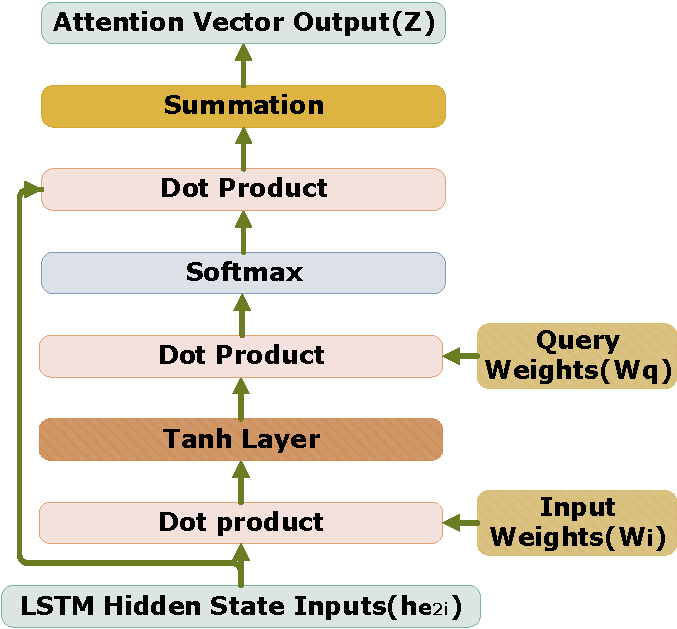
\includegraphics[scale=0.6]{att-layer}
	\caption{Context-aware Attention Network for the Model}
	\label{fig:att-layer}
\end{figure}
Attention layers come in broadly two flavors: \emph{soft} and \emph{hard} 
attention. The soft-attention uses weighted outputs of the input to 
\emph{attend} while hard-attention randomly selects a subset of the input to 
\emph{attend}. Each has its advantage and disadvantages, but we focus on the 
soft-attention method in this work. We sacrifice the efficiency of computation 
by using the weighted sum of all source inputs, as this helps the model to 
learn efficiently using backpropagation with gradient descent during training. 
Differing from \cite{salton2017attentive} that uses memory to create context, 
we add a query weight $W_q$ that is learned during training to ensure that each 
tuple is not attended to by just its occurrence in the present input sequence 
only but also based on its context throughout the training period. This query 
performs the similar role as the term-frequency inverse document frequency used 
to weigh the occurrence of tuples in the vector space model. \par
Fig. \ref{fig:att-layer} shows the connections of the attention layer 
block of Fig. \ref{fig:model-architecture}. The inputs the this layer are the 
input weights $W_i$ and the second layer encoder outputs $ h_{e2i} $. We pass 
the encoder output via a $\tanh$ layer after being scaled by the input weights 
$ W_i $ and the input bias vector $ b_i $ to generate correlation vectors $ 
m_i $ given in Equation \ref{eq:m-attention}.
\begin{equation}
\label{eq:m-attention}
	m_i = \tanh (W_{i} \cdot h_{e_2i} + b_i)
\end{equation}
This correlation vector (Equation \ref{eq:m-attention}) represents the effect 
of each input based on the present. Hence, we multiply it with the query vector 
$ W_q $ which has the global knowledge of each input tuple in the present 
input sequence to provide deep horizontally spanning inputs for the inference 
process as shown in Equation \ref{eq:q-vectors}. This vector is then passed 
through a softmax layer to generate $ s_i $ in Equation \ref{eq:softmax}. This 
normalized values is scaled by the input vectors $ h_{e_2i}$ and summed to 
generate the attention vector $ Z $ in Equation \ref{eq:z-context}.
\begin{align}
a_i &= W_{q} \cdot m_i + b_q \label{eq:q-vectors} \\
s_i &= \left( \frac{e^{a_i}}{\sum_j e^{a_j}}\right)_i \label{eq:softmax} \\
Z &= \sum_{i=1}^n s_i \times h_{e_2i} \label{eq:z-context}
\end{align}

\subsection{Fully Connected Layer}
\label{subsec:decoder}
Our significant architectural change from the previous \emph{encoder-decoder} 
frameworks is on what constitutes the input to the decoder. In most 
architectures that are recursive including that of \cite{bahdanau2014neural}, 
the past output target $ V_{t-1} $ only is the context which forms part of the 
input into the decoder for predicting $ V_t $. In our framework, we reason that 
while such $ V_{t-1} $ only as the context may be sufficient for natural 
languages which are more structured, logs which are semi-structured require 
more horizontal traversing contexts during the decoding process to improve the 
accuracy of the prediction. Hence, our decision to use the $ Z_{t-1}\, 
\text{and}\, V_{t-1} $ as context for decoding $ V_t $. Because the problem is 
formulated as a sequence-to-sequence problem, we posit that while $ V_{t-1} $ 
provides short term contexts in the decoder, the $ Z_{t-1} $ provides the much 
needed long term context required for accurate decoding of the output. In this 
design, $ h_{_di-1},V_{i-1} $ provide the context about decoded outputs while $ 
Z, Z_{i-1} $ provide the contexts about current and past attended inputs.  For 
a sequence reconstruction task like ours, the conditional probability is given 
in Equation \ref{eq:decoder} where $ k $ is a nonlinear function.
\begin{align}
P\left( \vec{V}\right) &= \prod_{i=1}^Ik\left(h_{_dt-1},V_{t-1},Z, 
Z_{t-1}\right) 
\label{eq:decoder}
\end{align}
The decoder output of Equation \ref{eq:decoder} is then passed through a 
fully-connected layer which produces the predicted output $V_t$ in the $t$ 
timestep.

\subsection{Anomaly Detection}
\label{subsec:anomaly}
Given $ \vec{x} \in \mathbb{Z}^{p} $ which serves as the input and target 
sequences, we aim to regenerate the $\vec{x}$ at the output by creating $ 
\vec{V} \in \mathbb{Z}^{p}$. Therefore, the perfect result is when $ 
\vec{x}_k  \equiv \vec{V}_k $ but this is hardly feasible because of the high 
randomness caused by interrupts and other events in the log traces. Hence, when 
we perform $ f:\vec{x}\mapsto \vec{V} $ given $ \vec{x} $ as the ground truths, 
the deviation $ \vec{d} = \abs{\vec{x} - \vec{V}} $ is the difference between 
the ground truth and the predicted value for the given sequence. This deviation 
becomes the prediction error values which we process further to decide if an 
anomaly has occurred or not. In our design, we use only the logs/traces from 
normal operating conditions of the system for training. To determine if an 
anomaly has occurred, we deviate from the approaches of 
\cite{malhotra2016lstm,malhotra2015long} by avoiding the use of threshold as 
that would form a hyperparameter which may be difficult to tune by users of the 
model. Rather, we use the prediction errors to model a Gaussian probability 
distribution and use confidence interval (CI) to determine if an anomaly 
has occurred. This CI method makes it easier for a non-professional to use and 
vary the \emph{CI} according to the safety level of an application.

\subsection{Distributed Model}
\label{subsec:distributed}
\begin{figure}[!t]
	\centering
	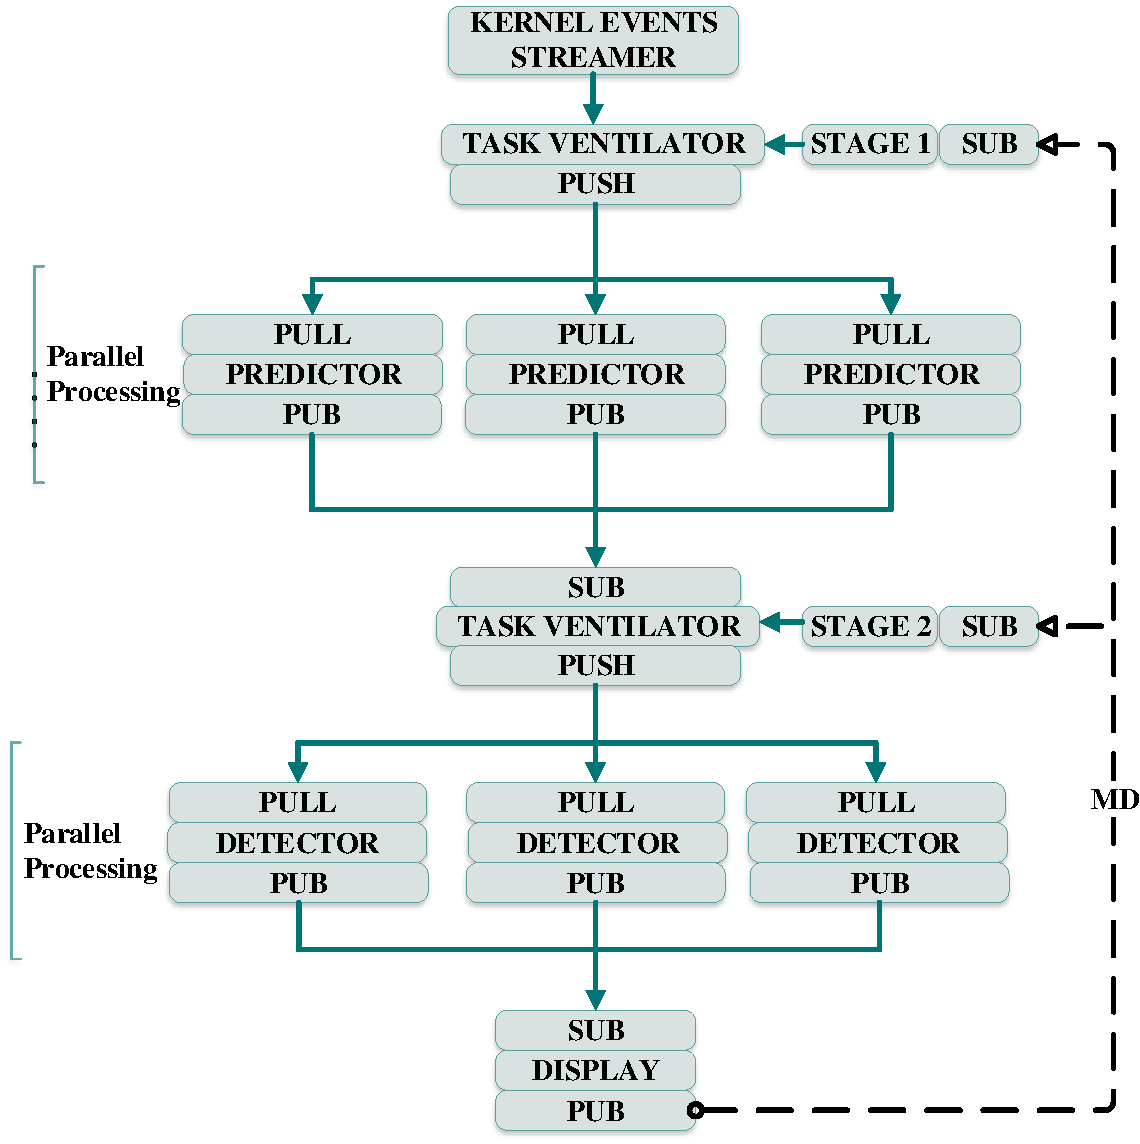
\includegraphics[scale=0.55]{decomposed-model}
	\caption{Deep Anomaly Model Showing both Concurrency and Decomposition}
	\label{fig:decomposed-model}
\end{figure}
Our model provides concurrency for multiple processes, and we distribute it 
between the embedded platform and a server. There are multiple ways of 
achieving parallelism, but we settled for the use of \emph{ZeroMQ} 
\cite{Akgul:ZEROMQ} as it helps to reduce the number of low-level use of locks, 
mutexes, and semaphores to provide conflict-free synchronization with no data 
corruption. \emph{Dealer, Router, Sub, Pub} shown in Figure 
\ref{fig:decomposed-model} are communication sockets and some of them are 
capable of asynchronous duplex communication.
\section{Experiments and Results}
\label{sec:experiments}

\section{Conclusions and Future Work}
\label{sec:conclusion}